% !TEX root = main.tex
\documentclass[a4paper, UKenglish, 11pt]{uiomaster}
\usepackage{lipsum}
\usepackage[subpreambles=true]{standalone}
\usepackage[table,xcdraw]{xcolor}


% MSE as loss function
% Training and testing, lr ?

\begin{document}
\chapter{DiLoc - A NN Apporach for Source Localization}
As mentioned in Chapter 1, an important topic in EEG signal analysis is the inverse problem, which aims to map measured EEG signals to localized equivalent current dipoles. This process is commonly referred to as source localization. In this chapter, we will introduce our feedforward neural network, named "DiLoc", created to solve such prosesses. We will provide a comprehensive overview of its parameters, architecture and training process. Moreover we will go through the simulation of the EEG signals for the the final dataset used for training. Additionally, we will present an alternative approach using a convolutional neural network for the same source localization.

\section{Architecture}
% Dropout 0.5
% Inializer ?
% Include neurons 
The development of DiLoc commenced with a deliberate and cautious approach, focusing on simplicity without compromising on accuracy in tackling diverse versions of the inverse problem. As a natural starting point, we adopted a fully connected, feed-forward neural network architecture, which eventually proved to be the most suitable framework for our purposes.

The input layer of DiLoc incorporates Rectified Linear Units (ReLU) as the activation function. This activation function introduces non-linearity into the model, enabling it to capture complex relationships and patterns within the data effectively. For the hidden layers, we employed the hyperbolic tangent (tanh) activation function. This decision was driven by its ability to squash input values into a range between -1 and 1, ensuring a smooth and differentiable transition during backpropagation. Conversely, in the output layer, we opted for a linear transformation without the use of any activation function. This setup allows the neural network to provide direct and unconstrained predictions for the x-, y-, and z-positions of the desired dipole source, as required in our application.

The determination of the number of hidden layers and neurons was carried out through a meticulous trial-and-error process. By experimenting with networks of varying complexities, i.e., small, medium, and large, we ultimately settled on the medium-sized network configuration. This choice, in conjunction with the selected activation functions, yielded the most promising results in terms of prediction accuracies.

The input layer is designed with 231 neurons, corresponding to the number of features in our dataset, i.e. the number of recording electrodes for each sample. Subsequently, the network consists of five hidden layers, comprising 512, 256, 128, 62, and 32 neurons, respectively. Finally, the output layer encompasses the three-dimensional coordinates (x, y, and z) representing the predicted position of the desired dipole source. Figure \ref{fig:FFNN_architecture} visualizes the construction of the fully connected neural network.

\begin{figure}[!htb]
    \centering
    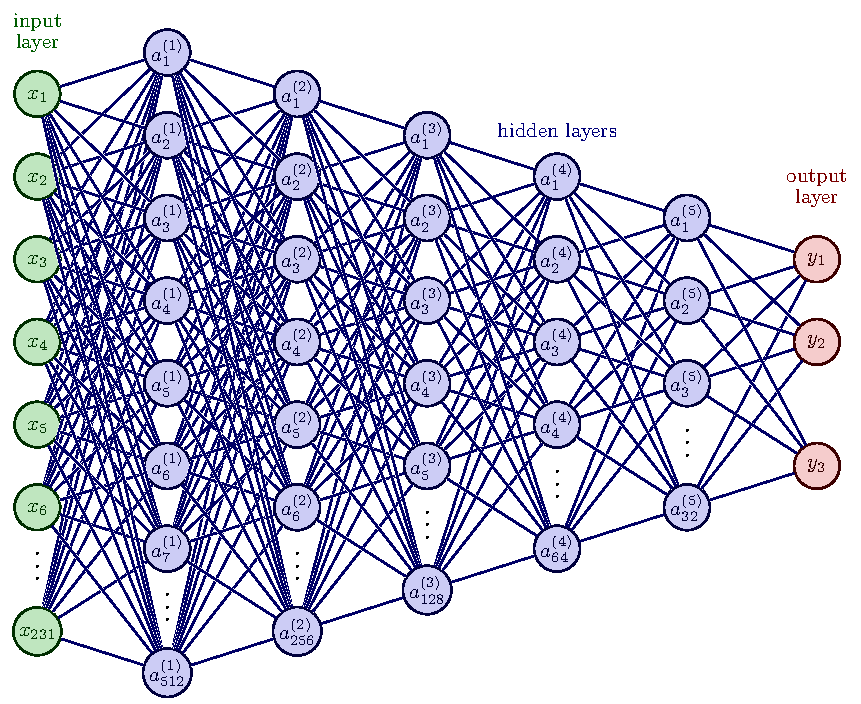
\includegraphics[width=\linewidth]{figures/FFNN_architecture.pdf}
    \caption{Architecture.}
    \label{fig:FFNN_architecture}
\end{figure}

\section{Simulation of EEG Signals}
The cortex matrix of the New York Head Model (NYHM) consists of 74,382 points, representing possible positions for localizing dipole sources. For training the neural networks, we utilize a dataset of self-simulated EEG measurements that correspond to the electromagnetic fields generated by these dipole sources. The dipole sources are randomly positioned within the cortex matrix. To simplify our problem, the amplitude of each dipole is fixed at $10^7$ nA $\mu$m. Additionally, in the case of single dipole source localization, the direction of the dipole moment is always rotated so that it is normal to the cerebral cortex. In some cases this will result in a dipole moment pointing perpendicular to the skull (directed towards an EEG electorde), while in other cases, due to the structure of the cortex, the dipole moment will point back into the cortex (but eventually towards an EEG electorde). The reason for this is that the human cortex is strongly folded, and the contribution to the EEG signal from a neural population (dipole moment) will depend on whether a dipole is located in a sulcus or a gyrus \cite{naess2021biophysically}. It is important to note that the EEG recordings capture a time series; however, for our analysis, we focus solely on the signal at t = 1, corresponding to the first time step. This allows us to examine the initial snapshot of the EEG signal's spatial distribution and its relationship to the dipole source locations within the cortex.
% Explain how this is done IR, looking for specific frequency ...

\subsection{The Effect of dipole location and orientation}
According to Naess et al. (2021) \cite{naess2021biophysically}, EEG signals are not particularly sensitive to small variations in the precise location of neural current dipoles. Despite the common belief that neurons in the upper cortical layers would dominate the EEG due to their proximity to the electrode compared to neurons in deeper layers, such location differences do not significantly affect the EEG signals. This phenomenon can be explained by the fact that the low conductivity of the skull introduces a spatial low-pass filtering effect, which mitigates the impact of location discrepancies.
% Maybe what is meant here is that we therefore only consider the outer corical surface

\begin{figure}[!htb]
    \centering
    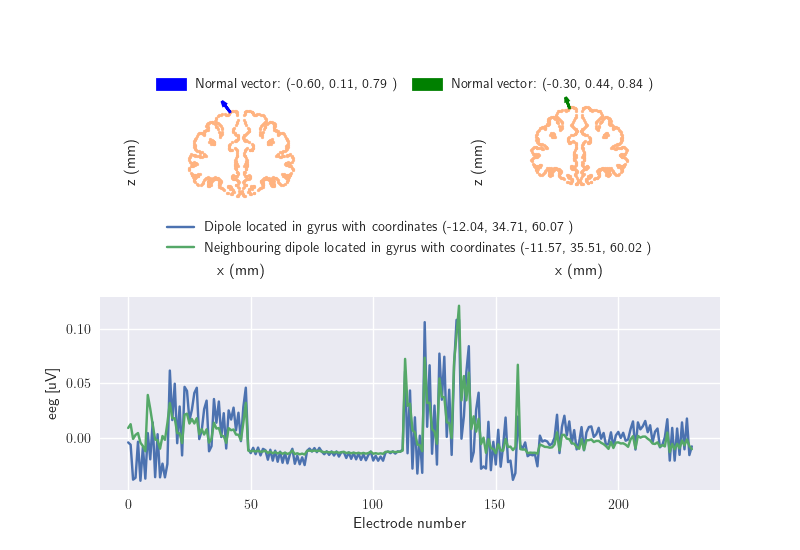
\includegraphics[width=\linewidth]{figures/neighbour_dipoles.png}
    \caption{EEG signal for neighbouring dipoles.}
    \label{fig:neighbour_dipoles}
\end{figure}

However, when considering the orientation of the dipoles relative to the EEG electrodes, the effect becomes noteworthy. To illustrate this, we present in Figure \ref{fig:gyrus_and_sulcus_EEG} the EEG signals obtained from two manually selected dipole locations within the New York head model. These dipoles are situated in a gyrus and a sulcus, respectively, resulting in distinct EEG outcomes. In general, the contribution of an individual current dipole to the EEG signal is maximized when the dipole is located perpendicularly within a gyrus, as depicted in Figure \ref{fig:gyrus_and_sulcus_EEG}B. On the other hand, if a dipole is placed in a sulcus with a perpendicular orientation, a significant EEG contribution can still be observed, but unlike the dipole in the gyrus, it exhibits a more dipolar pattern, as shown in Figure \ref{fig:gyrus_and_sulcus_EEG}C.

\begin{figure}[!htb]
    \centering
    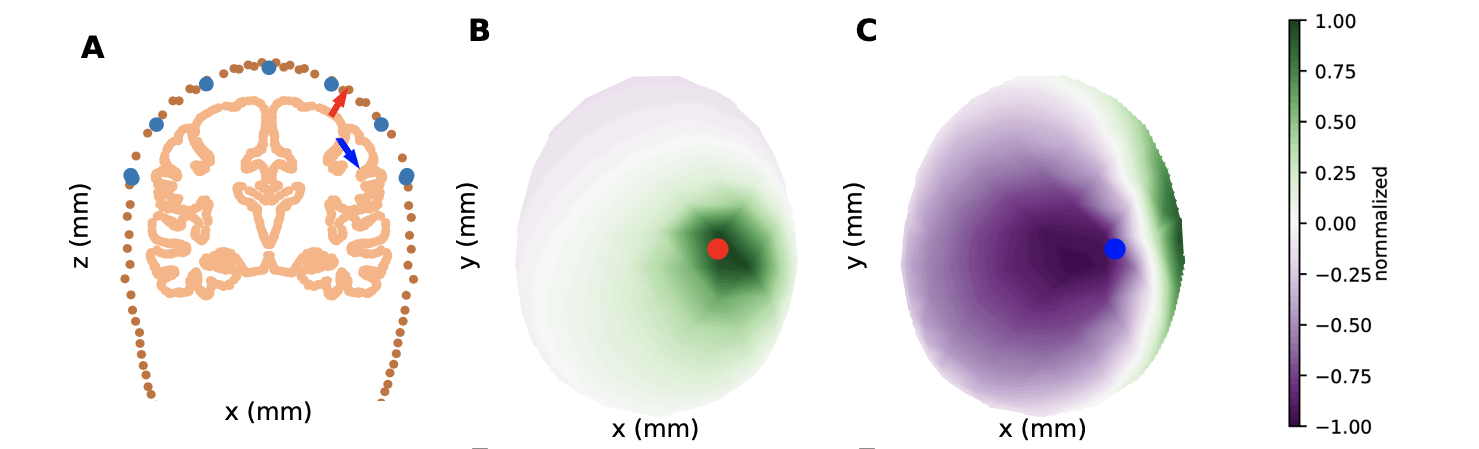
\includegraphics[width=\linewidth]{figures/gyrus_and_sulcus_EEG.png}
    \caption{A: Two selected dipole locations in the New York head model: one in a gyrus (red) and one in a sulcus (blue). The head model is viewed from the side (x, z-plane). Close to the chosen cross-section plane, EEG electrode locations are marked in light blue. Available dipole locations near the cortical cross-section form an outline of the cortical sheet and are marked in pink. The current dipole moment for all cases was $10^7$ nA$\mu$m. B: Interpolated color plot of EEG signal from the gyrus dipole, viewed from the top (x, y-plane). The plotted EEG signal is normalized, with a maximum value of 1.1 $\mu$V. C: Interpolated color plot of EEG signal from the sulcus dipole. The plotted EEG signal is normalized, with a maximum value of 0.7 $\mu$V. \cite{naess2021biophysically}}
    \label{fig:gyrus_and_sulcus_EEG}
\end{figure}

With other words, the EEG outcome is genuinely influenced by the orientation of the current dipole moment generating the signal, as variations in dipole orientation can impact both the direction and distribution of electrical potentials. In Figure \ref{fig:dipole_orientation}, we present the EEG signals obtained from four identical current dipoles with different orientations, situated in distinct hypothetical folding patterns of the cortical surface. Firstly, Figure \ref{fig:dipole_orientation}A and \ref{fig:dipole_orientation}C provide an expanded illustration of the aforementioned scenarios, incorporating additional dipole moments located in a gyrus and a sulcus, respectively. In Figure \ref{fig:dipole_orientation}B, where a collection of dipoles points randomly upwards and downwards, the EEG signal contribution appears to diminish significantly. Conversely, when the dipoles align in the depth direction of the cortex and are distributed across both gyrus and sulcus, we can expect an EEG contribution in between what we saw from Figure \ref{fig:dipole_orientation}A and \ref{fig:dipole_orientation}B, as depicted in Figure \ref{fig:dipole_orientation}D. Lastly, Figure \ref{fig:dipole_orientation}E demonstrates the minimal EEG contribution observed when the dipoles are divided between two opposing sulci.


\begin{figure}[!htb]
    \centering
    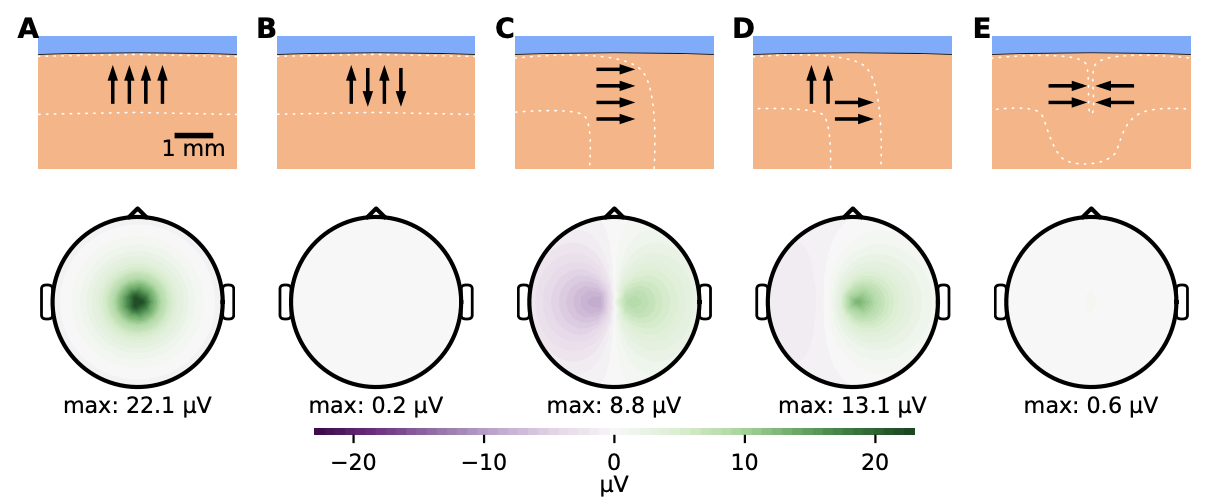
\includegraphics[width=\linewidth]{figures/dipole_orientation.png}
    \caption{Different folding patterns of the cortical surface are represented by white dashed lines. EEG signals are calculated from four identical current dipoles with varying orientations. A: Dipoles aligned in the same direction within a gyrus. B: Dipoles pointing in opposite directions within a gyrus. C: Dipoles aligned in the same direction within a sulcus. D: Dipoles distributed between a gyrus and a sulcus, pointing towards the cortical surface. E: Dipoles divided between opposing sulci, pointing towards the cortical surface.
    All panels have a dipole moment magnitude of 10 nAm, and the dipoles are positioned at the centers of the arrows in the top row.}
    \label{fig:dipole_orientation}
\end{figure}

% This is not the case for a simple dipole moment, but might be an issue when giving the populations a radii
% In our analysis, we simplify the scenario by considering one current dipole at a time, which allows us to avoid cancellations of potentials and obtain simpler EEG potentials. While this simplification may not capture the full complexity of neural activity, it provides us with a clearer understanding of the relationship between dipole orientation and EEG signals.


\subsection{Noise}
Experimental EEG recordings inevitably contain noise, which can interfere with the accurate analysis of brain activity. Artifacts, which are signals recorded by EEG but originating from sources other than the human brain, pose a particular challenge. Some artifacts can mimic genuine epileptiform abnormalities or seizures, underscoring the importance of identifying and distinguishing them from true brain waves \cite{sazgar2019eeg}.

Artifacts can be classified into two categories based on their origin. Physiological artifacts arise from the patient's own physiological processes, including ocular activity, muscle activity, cardiac activity, perspiration, and respiration. Technical artifacts, on the other hand, originate from external factors such as cable and body movements or electromagnetic interferences \cite{bitbrain}.

Filtering techniques are commonly employed to remove artifacts from EEG recordings prior to analysis. However, in the case of simulated EEG data, the need for artifact removal is eliminated as the data inherently lacks noise. Simulated EEG data can be considered as pre-filtered and preprocessed, ensuring a high signal-to-noise ratio (SNR) \cite{wiki-snr}. Nevertheless, to avoid overfitting and account for technical considerations, it is necessary to introduce noise to the data before feeding it into the neural network. This introduction of the noise is vital in order to make the trained neural network more likely to accurately handle real EEG recordings.

In our approach, we recognize that the introduction of noise to the simulated EEG data is an essential step to enhance the robustness of the trained neural network and ensure its ability to handle real EEG recordings effectively. Although the specific characteristics and quantity of noise have not been the primary focus of our study, we have opted for a straightforward approach. Our final dataset incorporates normally distributed noise with a mean of 0 and a standard deviation equal to 10$\%$ of the standard deviation observed in the simulated EEG recordings. By introducing this noise, we introduce random variations around each data point while preserving the overall normalization properties of the dataset.

\begin{figure}[!htb]
    \centering
    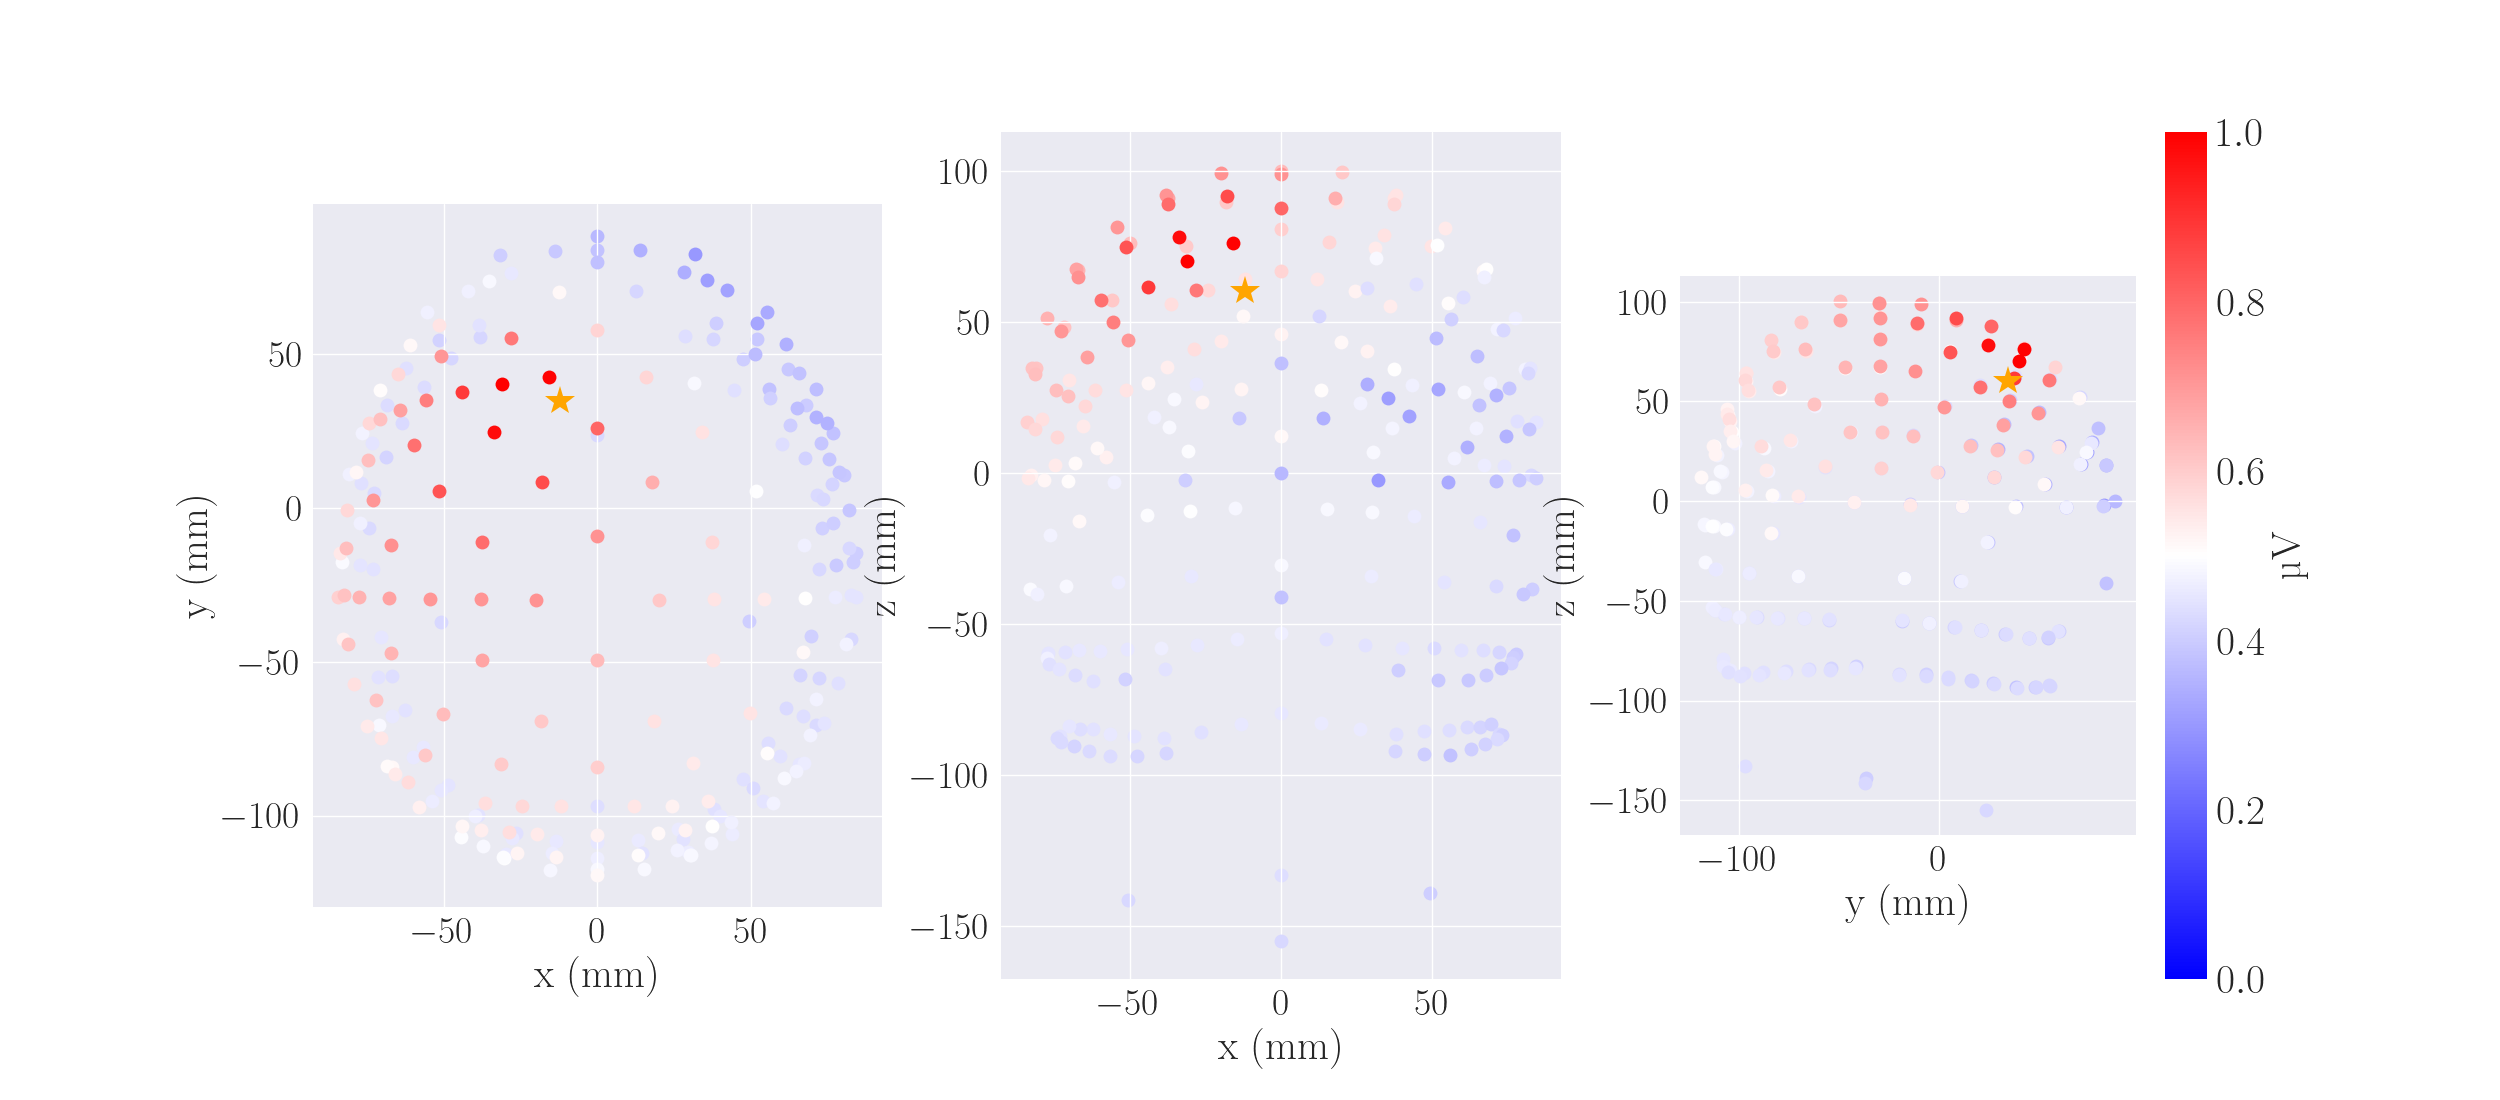
\includegraphics[width=\linewidth]{figures/simple_dipole_eeg_field_noise_10.png}
    \caption{EEG for a sample containing one single current dipole source at a random position within the celebral cortex. As for all samples, 10 percent of normally distributed noise has been added to the original signal. The EEG measure is seen from both sides (x-, z-plane and y-, z-plane) and above (the x-, y-plane). EEG electrode locations are presented as filled circels, where the color of the fill represents the amplitude of the measured signal for the given electrode. The position of the current dipole moment is marked with a yellow star.}
    \label{fig:eeg_field_1_dipole_example}
\end{figure}

\subsection{Final Dataset}
The final dataset comprises 70 000 rows, where each row corresponds to a single sample or patient. Within the dataset, there are 231 columns representing the features, which denote the EEG measurements recorded at each electrode. Consequently, the design matrix has a size of 70 000 x 231. In practice, the design matrix consists of pairs of input vectors with EEG signals and corresponding output vectors, where the answer key is the x-, y- and z coordinate of different dipole sources.

Figure \ref{fig:eeg_field_1_dipole_example} presents an example of the input EEG data for a single sample, with 10$\%$ noise added. The illustration showcases the EEG results obtained from a sample containing a solitary current dipole source positioned randomly within the cerebral cortex. The dipolar pattern in the figure indicates that the dipole is located within a sulcus. The EEG measure is visualized from multiple perspectives, including the x-z plane, y-z plane, and the x-y plane. The electrode locations are represented by filled circles, with the color of the fill indicating the amplitude of the measured signal at each electrode. The position of the current dipole moment is denoted by a yellow star. As observed from the figure, the EEG signal for this specific sample ranges from -1 to 1 $\mu$V.

% Before being feed to the DiLoc network for training, the data is splitted into train, validation and test parts. The train- and validation data are the batches of the data set that the network uses during training. Out of the 70 000 samples in the final dateset, 50000 is set off to the purpose of train and validation data. Out of these 50000 sampes, randomly selected 80 percent of the rows are put into the training set. The remaining 20 percent operates as the validation set, which is useful in order to prevent the network to overfit during training. The test set which contains the final 20 000 samples will be used after the training prosess for the purpose of testing how well the model generalizes to new, unseen data.

Prior to being fed into the DiLoc network for training, the dataset was splittied into distinct segments: the train, validation, and test sets. This partitioning is vital for assessing and optimizing the network's performance. Among the 70 000 samples in the final dataset, 50 000 samples are designated for the train and validation data. To ensure a representative and unbiased allocation, 80 percent of these 50 000 samples are randomly assigned to the training set. This training set serves as the core data that the network utilizes during the training process. The remaining 20 percent of the 50 000 samples form the validation set. This set plays the role in preventing overfitting, the phenomenon where the network becomes excessively attuned to the training data and consequently performs poorly on new data. By independently evaluating the model's performance on the validation set throughout training, we can fine-tune the network's parameters to achieve better generalization to unseen data. Once the network completes its training process, the test set comes into play. Comprising 20 000 samples, the test set serves as the benchmark for assessing the model's ability to generalize and make accurate predictions on new data instances. By adhering to this rigorous train-validation-test data partitioning, we ensure a robust evaluation of the DiLoc model's performance and its capacity to effectively handle real-world scenarios with previously unseen data.


\section{Training the DiLoc Network}
To train the DiLoc network efficiently, several key techniques are employed, including stochastic gradient descent (SGD), mean squared error (MSE) as the cost function, learning rate scheduling, and L1 and L2 regularization. Detailed explanations of these techniques can be found in the Chapter 3.

The objective during training is to find the optimal parameters $\beta$ that minimize the cost function. The cost function represents the discrepancy between the network's predictions and the actual target values. By iteratively updating the parameters to minimize the cost function, the network fine-tunes its internal representations to make more accurate predictions. MSE is chosen as the cost function for the DiLoc network, as it provides a smooth and continuous measure of the model's performance during training, penalizing larger errors more heavily.

% Include why we went for batch size 32 and mom = 0.35 (instead of 0.9)
Optimizers play a crucial role in reducing the network's loss and providing accurate results. In this case, SGD with momentum is utilized as the network's optimizer. SGD with momentum enhances the sensitivity of the network to initialized weights and provides fast convergence. The algorithm uses mini-batches of size 32, introducing fluctuation to the data and preventing the network from getting stuck in local minima or saddle points. The momentum hyperparameter, set to 0.35 in this context, helps reduce high variances in the optimization process and accelerates convergence towards the right direction, leading to faster training.

To improve the training process further, learning rate scheduling is employed. This technique adjusts the learning rate over time, allowing the network to take larger steps in the early stages and gradually decrease the learning rate as it approaches convergence. The initial learning rate is set to 0.001, and is further decreased, which provides balance between rapid convergence in the initial phases and fine-tuning towards the end.

Additionally, L1 and L2 regularization techniques are incorporated as optional parameters into the DiLoc network. These regularization methods help prevent overfitting and improve generalization to unseen data. By adding penalty terms to the cost function, L1 and L2 regularization encourage the model to favor simpler and more generalizable solutions.

After the DiLoc network is fully trained on the training dataset, it has learned the optimal parameters to make accurate predictions. The model's performance is evaluated using a separate test dataset, which the network has not seen during training. This test data provides an unbiased assessment of the model's accuracy and its generalization capabilities to unseen data.

In the upcoming chapters, we will present different approaches to the inverse problem and showcase the performance of the DiLoc network across these approaches. The evaluation results will demonstrate the effectiveness and utility of the trained model in solving the localization task for various scenarios.

\section{Diloc as Convolutional Neural Network}

\end{document}